\documentclass{math}

\usepackage{graphicx}

\geometry{letterpaper, margin=0.5in}

\title{Intro to Computer Science Theory: Homework 2}
\author{Alvin Lin}
\date{August 2017 - December 2017}

\begin{document}

\maketitle

\subsection*{Problem 1}
Give FA state transition diagrams for the following languages. Be sure to label
the names of your states. Each language is over the alphabet \( \{a,b\} \),
and is defined as the set of all strings.
\begin{enumerate}
  \item that begin or end in \( aa \) in \( bb \).
    \begin{center}
      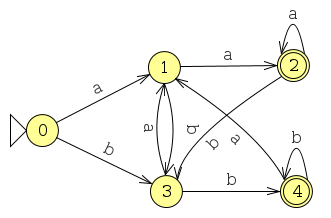
\includegraphics[width=8cm]{assets/hw_02_1_1.png}
    \end{center}
  \item that do not have \( aaa \) as a substring.
    \begin{center}
      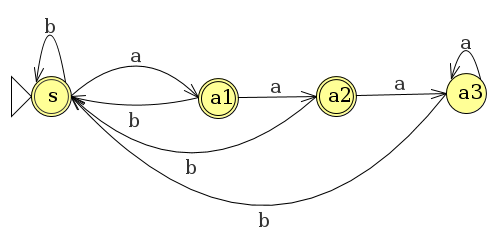
\includegraphics[width=10cm]{assets/hw_02_1_2.png}
    \end{center}
  \item that contain both \( aba \) and \( bab \) as substrings.
    \begin{center}
      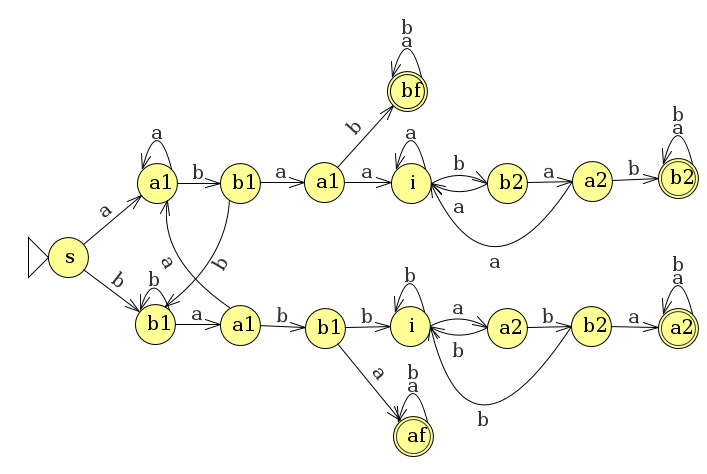
\includegraphics[width=15cm]{assets/hw_02_1_3.png}
    \end{center}
  \item whose length is a multiple of 5.
    \begin{center}
      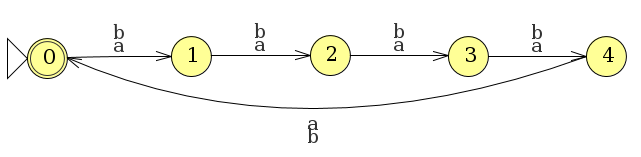
\includegraphics[width=12cm]{assets/hw_02_1_4.png}
    \end{center}
  \item where the number of \( a \)'s after the last \( b \) in the string is
    odd.
    \begin{center}
      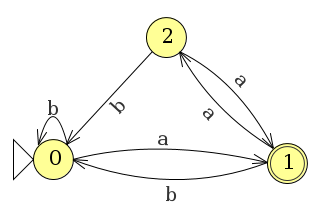
\includegraphics[width=8cm]{assets/hw_02_1_5.png}
    \end{center}
\end{enumerate}

\subsection*{Problem 2}
Provide formal definitions for 1, 4, and 5 above. Try to make them as concise
as possible.

\subsubsection*{Finite Automaton 1}
\( M = \{Q,\Sigma,\delta,0,\{2,4\}\} \) where:
\begin{itemize}
  \item \( Q = \{0,1,2,3,4\} \)
  \item \( \Sigma = \{a,b\} \)
  \item \( \delta: Q\times E\to Q \) is defined on \( (q,z)\in Q\times\Sigma \) as:
    \[ \delta(q,x) = \begin{cases}
      1 & if\ (x = a) \wedge (q\in\{0,3,4\}) \\
      2 & if\ (x = a) \wedge (q\in\{1,2\})   \\
      3 & if\ (x = b) \wedge (q\in\{0,1,2\}) \\
      4 & if\ (x = b) \wedge (q\in\{3,4\})
    \end{cases} \]
\end{itemize}

\subsubsection*{Finite Automaton 4}
\( M = \{Q,\Sigma,\delta,0,\{0\}\} \) where:
\begin{itemize}
  \item \( Q = \{0,1,2,3,4\} \)
  \item \( \Sigma = \{a,b\} \)
  \item \( \delta: Q\times E\to Q \) is defined on \( (q,z)\in Q\times\Sigma \) as:
    \[ \delta(q,x) = q+1 \]
\end{itemize}

\subsubsection*{Finite Automaton 5}
\( M = \{Q,\Sigma,\delta,0,\{1\}\} \) where:
\begin{itemize}
  \item \( Q = \{0,1,2\} \)
  \item \( \Sigma = \{a,b\} \)
  \item \( \delta: Q\times E\to Q \) is defined on \( (q,z)\in Q\times\Sigma \) as:
    \[ \delta(q,x) = \begin{cases}
      0 & if\ (x = b) \\
      q+1 & if\ (x = a) \wedge (q \ne 2) \\
      1 & if\ (x = a) \wedge (q = 2)
    \end{cases} \]
\end{itemize}

\section*{Problem 3}
Prove, in the following steps, that for any language \( L \), if
\( L\circ L\subseteq L \) then \( L = \{\epsilon\} \) or \( L \) is
infinite.
\begin{enumerate}
  \item Write the theorem using quantifiable logic, as in our previous
    homework.
    \[ (L\circ L\subseteq L)\to((L =
      \{\epsilon\}) \vee L \text{ is infinite}) \]
  \item Rewrite the following statement in quantifiable logic. For all natural
    numbers \( n \), there exists an \( x \) in \( L \) such that \( |x|>n \).
    Note that this is effectively what it means for \( L \) to be infinite.
    \[ \forall{n}(n\in\N)\exists{x}(x\in L\wedge |x|>n) \]
  \item Where appropriate, substitute into your answer in 1 for the definitions
    of \( \circ,\subseteq \), and ``L is infinite''.
    \[ \forall{x}((x\in L\circ L)\to(x\in L))\to((L =
      \{\epsilon\})\vee(\forall{n}(n\in\N)\exists{x}(x\in L\wedge |x|>n))) \]
  \item Write the following statements in predicate logic.
    \begin{enumerate}
      \item For any string \( x \), \( |x| = 0 \) if and only if
        \( x = \epsilon \).
        \[ \forall{x}(|x| = 0)\leftrightarrow(x = \epsilon) \]
      \item For any strings \( x \) and \( y \), \( |xy| = |x|+|y| \).
        \[ \forall{x}\forall{y}(|xy| = |x|+|y|) \]
    \end{enumerate}
\end{enumerate}

\begin{center}
  If you have any questions, comments, or concerns, please contact me at
  alvin@omgimanerd.tech
\end{center}

\end{document}
